\documentclass[oneside,a4paper,12pt]{article}
\usepackage{graphicx}
\usepackage[section]{placeins}
\usepackage{listings}
\graphicspath{{~/templates/}, {../images/}}

\makeindex
\begin{document}
	\begin{titlepage}
		\includegraphics[width=4cm]{logopopo.png}
		\hspace*{\fill}
		\includegraphics[width=6cm]{univlille.png}
		
		\begin{center}
			\vspace{1cm}
			\textbf{TP Traitement du Signal}\\
			\textbf{Correlation Numérique}\\
			\vspace{1cm}
			\textbf{Valentin DOSIAS, Maxence NEUS}\\
			\vspace{3cm}
			%\includegraphics[width=13cm]{titlepage.png}\\
			\vspace{\fill}
			\textbf{Decembre 2021}\\
		\end{center}
	\end{titlepage}
	
	\tableofcontents
	\newpage
	
	\section{Introduction}
	
	La corrélation numérique est utilisée lorsque l’on recherche la relation entre deux processus. L’objectif de ce TP est de d’utiliser deux méthodes de corrélation numériques pour traiter quelques applications. Tout d’abord, nous allons utiliser l’inter-corrélation sur deux signaux simples puis nous allons utiliser l’auto-corrélation pour obtenir la réponse impulsionnelle d’un système.
	
	\section{Inter-corrélation numérique}
	
	Pour l’inter-corrélation, nous allons travailler avec deux signaux sinus. Ces deux sinus auront même fréquence, même amplitude mais l’un sera déphasé par rapport à l’autre.
	
	\begin{figure}[h]
		\centering
		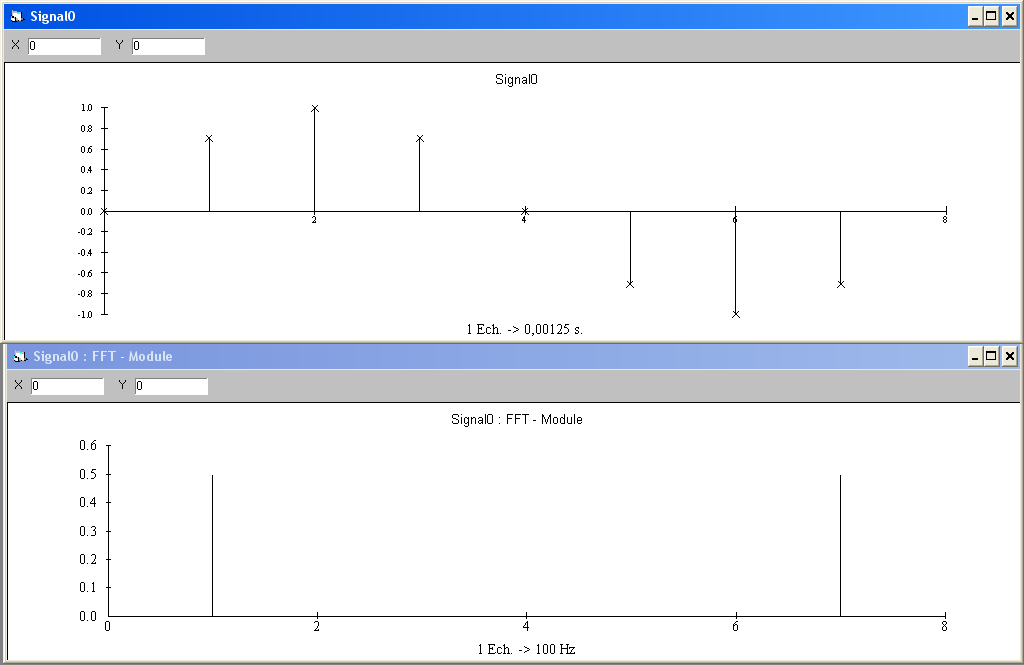
\includegraphics[width=13cm]{fig1.png}
		\caption{Préparation}
	\end{figure}
	
	En théorie, nous avons la phase à l’origine $\phi_{0}$ qui n’a aucune influence sur le résultat de la corrélation des deux signaux. Cependant le déphasage du deuxième signal $\phi$ à une influence et devrait apparaître sur le signal de sortie.\\
	
	Nous allons donc vérifier ces observations sur le logiciel Easy Curve.\\
	
	Nous choisissons deux sinus ayant une fréquence de 100 Hz, une amplitude de 1 Volt et le deuxième signal est déphasé de 45°. Nous avons d’abord essayé de discrétiser ces signaux avec une fréquence d'échantillonnage de 1000 Hz et de 16 échantillons.\\
	
	Nous obtenons les signaux ci-dessous.
	\begin{figure}[h]
		\centering
		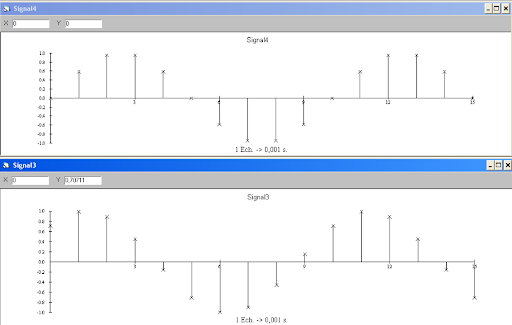
\includegraphics[width=10cm]{fig2.png}
		\caption{Signaux 1 et 2}
	\end{figure}

	Nous obtenons la corrélation suivante.
	
	\begin{figure}[h]
		\centering
		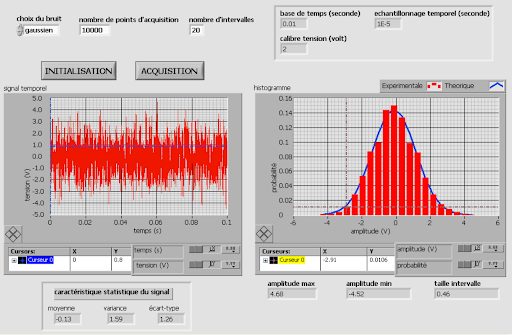
\includegraphics[width=10cm]{fig3.png}
		\caption{Correlation de 1 et 2}
	\end{figure}

	Ce n’est pas le résultat attendu, la fréquence d'échantillonnage est trop faible.
	Nous avons ensuite augmenté le nombre d’échantillons à 128 et la fréquence d'échantillonnage à 12800 Hz. Nous obtenons les signaux ci-dessous.
	
	\begin{figure}[h]
		\centering
		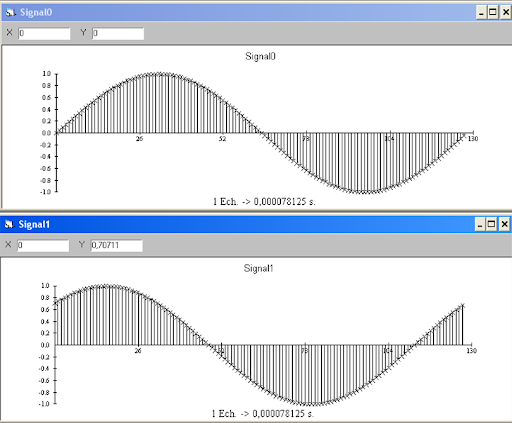
\includegraphics[width=10cm]{fig4.png}
		\caption{Signaux 1 et 2 à haute fréquence d'echantillonage}
	\end{figure}

	Une fois les deux signaux corrélés, nous obtenons le signal suivant.
	
	\begin{figure}[h]
		\centering
		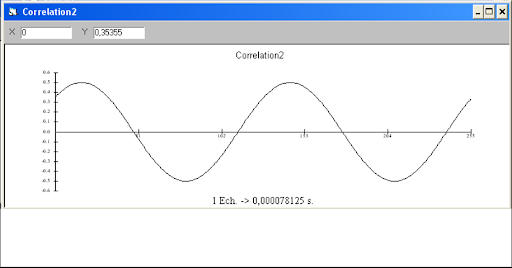
\includegraphics[width=10cm]{fig5.png}
		\caption{Correlation de 1 et 2}
	\end{figure}

	Ce résultat en bien en accord avec la théorie, nous avons bien une amplitude de 0.5V soit la moitié de l’amplitude des signaux de départ. Nous retrouvons aussi le déphasage de 45° du deuxième signal. Ainsi la fréquence d'échantillonnage nous permet de discrétiser correctement notre sinus pour être reconnu comme tel et plus nous avons un nombre d’échantillons importants plus le logiciel sera précis sur la corrélation et le signal de sortie sera “lissé”.
	
	\section{Obtention de la réponse impulsionnelle d’un système}
	
	\paragraph{}
	Un générateur à bruit blanc délivre un signal dont le spectre comporte des raies d’amplitude unitaire à toutes les fréquences alors que le générateur de bruit rose comporte des raies d’amplitude unitaire jusqu’à une certaine fréquence. Il suffit donc de prendre une fréquence maximale de bruit assez grande par rapport à la fréquence de coupure du système car au dessus de cette fréquence la réponse impulsionnelle du système sera nulle.
	\paragraph{}
	La densité spectrale de puissance peut se calculer en faisant la transformée de Fourier de l’autocorrélation d’un signal. La fonction d’autocorrélation du bruit nous est donnée dans le sujet. La transformée de Fourier est une opération linéaire, nous pouvons donc décomposer la fonction en une somme de deux signaux simples.
	
	Nous avons donc la constante négative $-\frac{A^{2}}{L}$ de TF un pic de Dirac d’amplitude $-\frac{A^{2}}{L}$ Nous avons aussi un triangle de formule $\frac{(L+1)A^{2}}{L}$ et donc de transformée de Fourier :
	$$ \frac{(L+1)A^{2}}{L}*\theta*sin^{2}(\pi f \theta) $$
	La densité spectrale de puissance vaut donc :  
	$$ S(f)= \frac{(L+1)A^{2}}{L}*\theta*sin^{2}(\pi f \theta) - \frac{A^{2}}{L}*\delta(f)$$
	
	\begin{figure}[h]
		\centering
		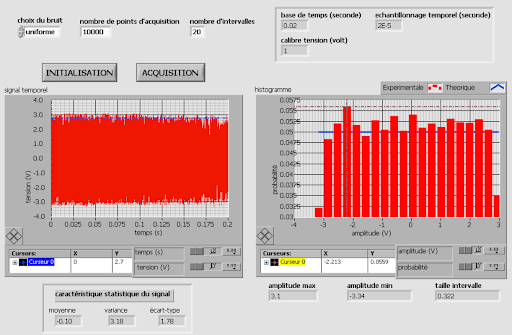
\includegraphics[width=9cm]{fig6.png}
		\caption{Allure de la DSP}
	\end{figure}

	Nous générons maintenant un bruit rose à l’aide du logiciel avec une fréquence d'échantillonnage de 300 Hz et n=6.\\
	
	\begin{figure}[h]
		\centering
		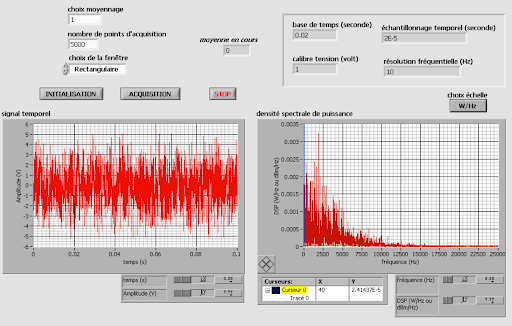
\includegraphics[width=10cm]{fig7.png}
		\caption{Bruit}
	\end{figure}

	Nous avons fait l’autocorrélation pour 3 bruits rose différents.
	\begin{figure}[h]
		\centering
		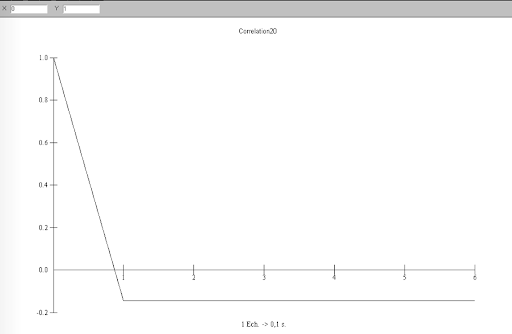
\includegraphics[width=10cm]{fig8.png}
		\caption{f=10hz, n=3 et A=1}
	\end{figure}
	\begin{figure}[h]
		\centering
		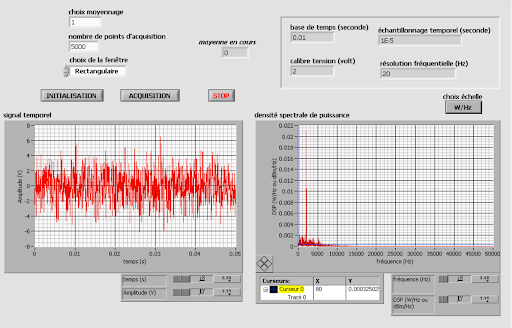
\includegraphics[width=11cm]{fig9.png}
		\caption{f=300 hz, n=6 et A=1}
	\end{figure}
\newpage
	\begin{figure}[h]
		\centering
		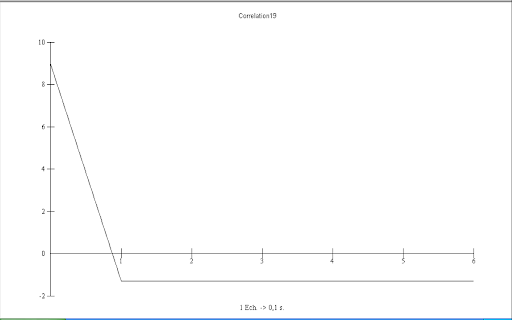
\includegraphics[width=11cm]{fig10.png}
		\caption{f=10 hz, n=3 et A=3}
	\end{figure}
	\begin{figure}[h]
		\centering
		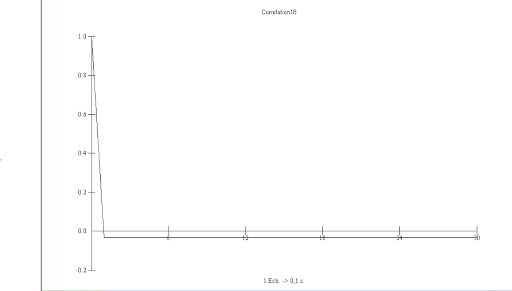
\includegraphics[width=12cm]{fig11.png}
		\caption{f=10 Hz, n=5 et A=1}
	\end{figure}
	\newpage
	
	
	\paragraph{}
	Ainsi, nous avons constaté que lorsque le nombre de bascules augmentent ici n, $\theta$ diminue tandis que L et T augmentent. En effet, plus nous augmentons n, plus le logiciel est précis et plus nous nous rapprochons d’un pic de Dirac. Cependant, il ne faut pas prendre un nombre de bascules trop grand sinon le logiciel plante. Lorsque nous augmentons la fréquence d'échantillonnage, l'échelle change donc diminue aussi la période de l’horloge $\theta$.
	
	\section{Réponse impulsionnelle circuit RC}
	
	On va utiliser notre générateur de bruit pour déterminer la réponse inpultionnelle d'un filtre RC, pour cela on va utiliser un correlateur. On peut montrer que si l'entrée du filtre est un bruit blanc, alors la correlation de cette entrée et de la sortie du filtre donne la réponse impultionnelle de ce filtre.\\
	$$ s(t) = h(t)*e(t) $$
	$$ alors: C_{es} = s(t)*e(-t)$$
	$$ donc: C_{es} = h(t)*e(t)*e(-t) $$
	$$ or: e(t)*e(-t) = C_{ee} $$
	$$ Comme: C_{ee}=\delta(t), alors: C_{es} = h(t) $$
	
	On a donc réalisé la correlation de e et s et on a réalisé une transformation pour obtenir le diagramme de baude du filtre.
	
	\begin{figure}[h]
		\centering
		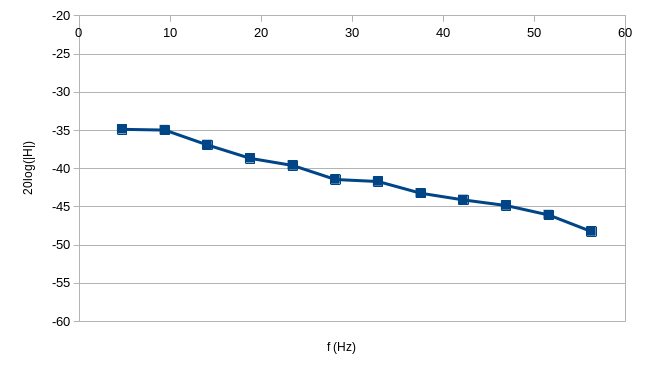
\includegraphics[width=12cm]{fig12.png}
		\caption{Diagramme de baude du filtre}
	\end{figure}

	On avait choisi notre filtre de façon à avoir une fréquence de coupure à 16Hz, on peut lire sur le diagramme de baude que le gain passe à $Gain_{max}-3dB$ entre les échantillons à 14 et 18Hz, ce qui correspond à la fréquence de coupure attendue.
	
	\section{Conclusion}

	On a vu au cours de ce TP comment il est possible de simuler les auto-correlations de différents signaux. On a également vu comment on peut déterminer la réponse impultionnelle d'un filtre quelconque.\\

\end{document}